\begin{frame}
\frametitle{Espace d'approximation / Points de volume}
\vfill
\begin{columns}[c]
\column{.5\textwidth}
\begin{itemize}
\item Ordre d'interpolation $\Deg \in \EnsN^\star$ ;
\item $(\Deg + 1)^3$ points et poids d'intégration de Gauss-Legendre :
\begin{align*}
&(\GLN{i})_{i \ge 0} \subset \HexaRef , \\
&(\GLW{i})_{i \ge 0} \subset \EnsR^{\star +} \ ;
\end{align*}
\item Formule de quadrature volumique :
\begin{align*}
\int_{\HexaRef} \psi (\xref) d\xref \approx
	\sum_{i} \GLW{i} \psi (\GLN{i}) .
\end{align*}
\end{itemize}
\column{.5\textwidth}
\begin{figure}
\centering
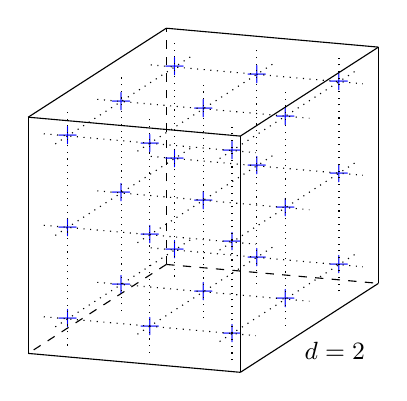
\begin{tikzpicture}[scale=3,rotate around x=270,rotate around z=258]
	% cube arriere
	\draw [dashed] (0,0,0) -- (1,0,0);
	\draw [dashed] (0,0,0) -- (0,1,0);
	\draw [dashed] (0,0,0) -- (0,0,1);

	\draw (0.7,1.25) node {\small$d=2$};

	% gauss legendre: 0.1127, 0.5, 0.8873
	\def \pgs {0.1127,0.5,0.8873}

	% points volumiques
	\foreach \x in \pgs {
	\foreach \y in \pgs {
	\foreach \z in \pgs {
		\draw (\x,\y,\z) node[blue] {$\bm{+}$};
	}}}
	% lignes pointilées direction x
	\foreach \y in \pgs
	\foreach \z in \pgs {
		\draw [dotted] (0,\y,\z) -- (1,\y,\z);
	}
	% lignes pointilées direction y
	\foreach \x in \pgs
	\foreach \z in \pgs {
		\draw [dotted] (\x,0,\z) -- (\x,1,\z);
	}
	% lignes pointilées direction z
	\foreach \x in \pgs
	\foreach \y in \pgs {
		\draw [dotted] (\x,\y,0) -- (\x,\y,1);
	}

	% cube avant
	\draw [-] (1,1,0) -- (1,0,0);
	\draw [-] (0,1,1) -- (0,1,0);
	\draw [-] (1,0,1) -- (0,0,1);

	\draw [-] (1,1,0) -- (0,1,0);
	\draw [-] (0,1,1) -- (0,0,1);
	\draw [-] (1,0,1) -- (1,0,0);

	\draw [-] (1,1,0) -- (1,1,1);
	\draw [-] (0,1,1) -- (1,1,1);
	\draw [-] (1,0,1) -- (1,1,1);
\end{tikzpicture}
\end{figure}
\end{columns}
\vfill
\end{frame}

